\chapter{Linear Dimensionality Reduction}

As presented in the previous sections, data sets with many features may present a series of issues: difficult visualization, high performance requirements, noise etc. In this section, it will be discussed methods related with linear dimensionality reduction, i.e., the shrinking of data sets by transformation and/or removal of features, while minimizing information loss.

Consider the data set $K$. $K$ has its samples expressed by two similarly scaled dimensions. It is clear, however, that the samples follow a very particular distribution:

\begin{figure}[H]
    \centering
	\captionsetup{justification=centering}

	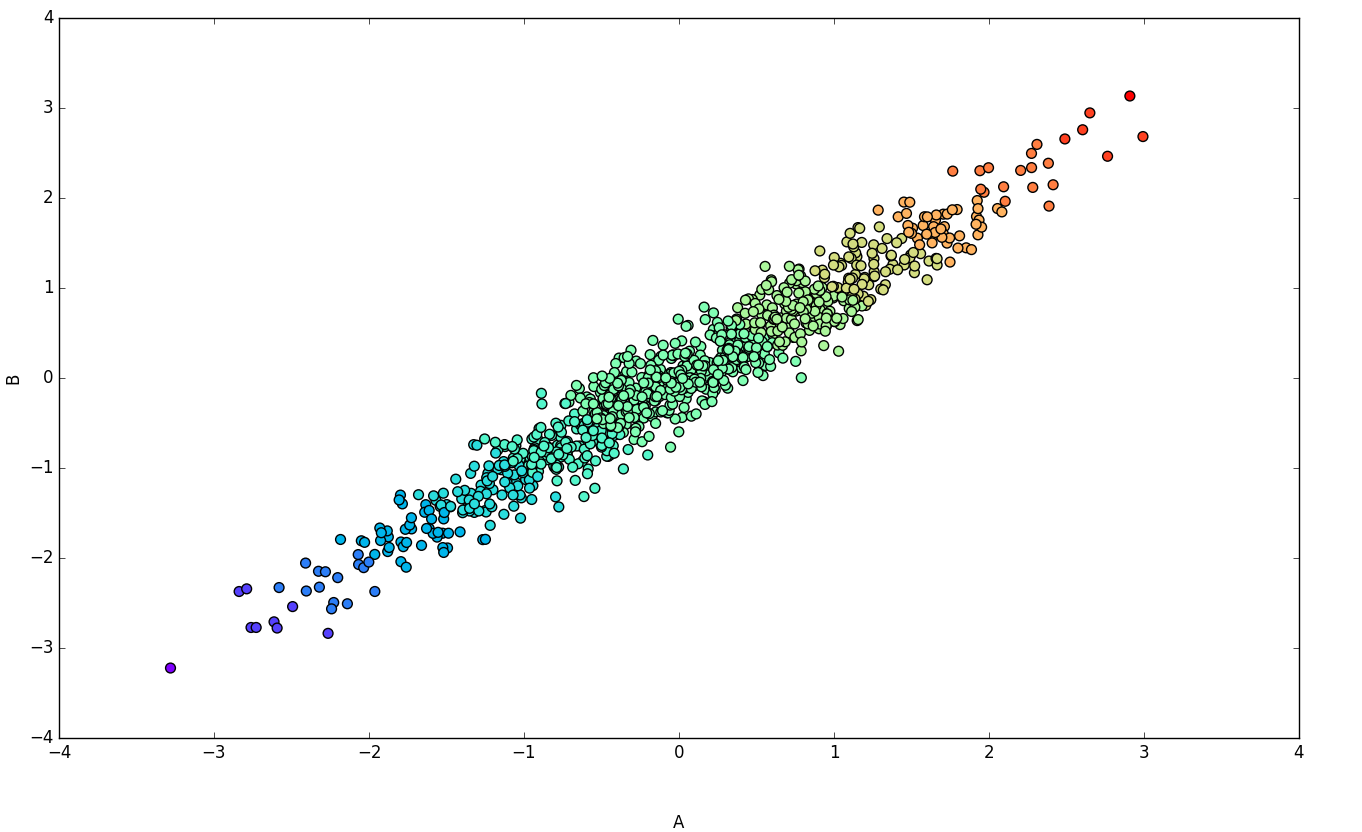
\includegraphics[width=.8\linewidth]{datasets/r}
	\caption{The data set $K \in \mathbb{R}^2$.}
	\label{fig:datasetr}
\end{figure}

Additionally, something interesting can be observed when analyzing the covariance matrix of $K$: as it is not a diagonal matrix, the variance of $x$ from its mean somehow correlates with the variance of $y$. \cite{pcajon2003}

\begin{table}[H]
	\centering
	\begin{tabular}{|c|c|c|}
		\hline
			& \textbf{x} & \textbf{y} \\\hline
		\textbf{x} & 1.26682132  & 1.29158697 \\\hline
		\textbf{y} & 1.29158697  & 1.40358478 \\\hline
	\end{tabular}
	\caption{Covariance between the components of $K$.}
\end{table}

\section{Principal Component Analysis}

As in $K$, some data sets follow certain distributions that are majorly contained in a few orthogonal components, where a component is the result of a linear combination of the original features.

Principal Component Analysis (PCA) is a statistical technique that attempts to transform a $n$-dimensional data set $X$ into a $m$-dimensional data set $Y$, where, hopefully, $k \ll n$. Furthermore, the dimensions of $Y$ will necessarily be orthogonal components aligned with the direction in which the variance of samples in $X$ is maximum, commonly referred to as \textbf{principal components}. \cite{pca1989} In figure \ref{fig:datasetrpc}, the orange and purple vectors are the principal components of the data set $K$.

\begin{figure}[H]
	\centering
	\captionsetup{justification=centering}
	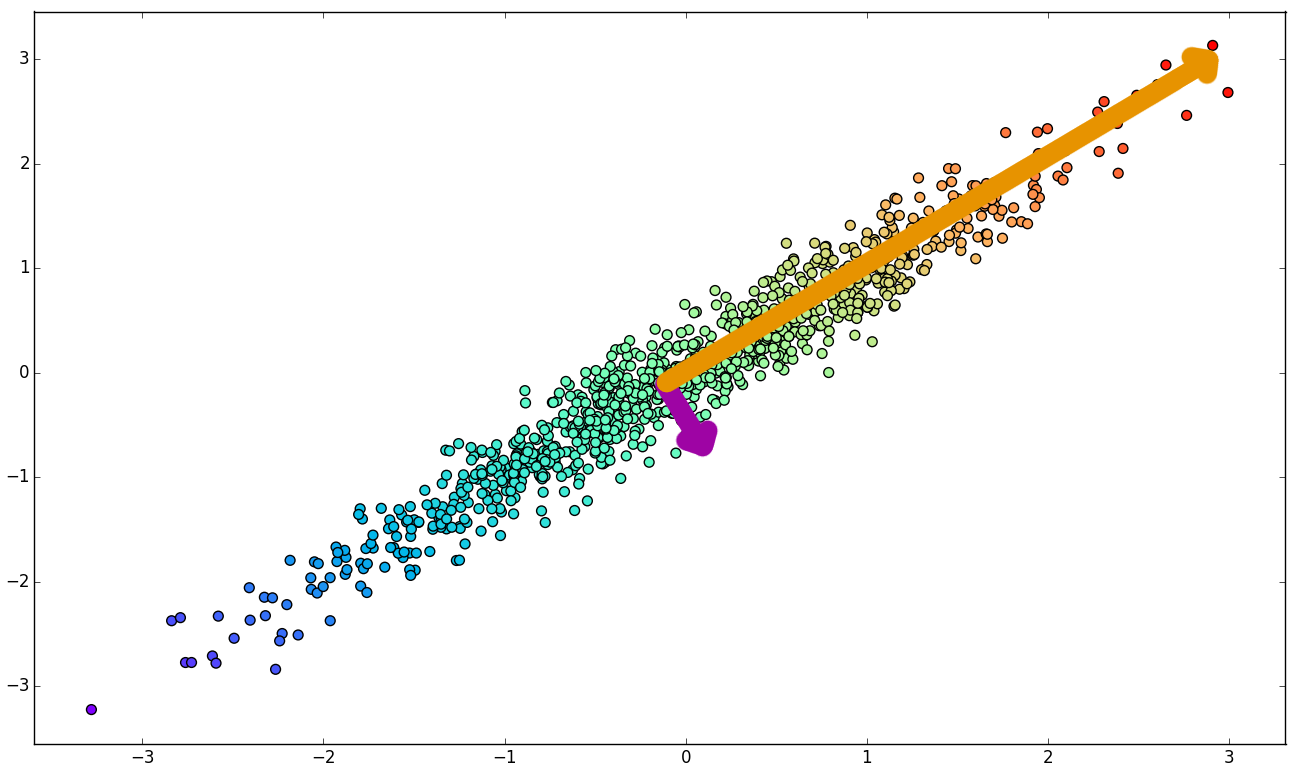
\includegraphics[width=.8\linewidth]{datasets/r_pcs}
	\caption{The principal components of $K$.}
	\label{fig:datasetrpc}
\end{figure}

\subsection{Study of the PCA Algorithm}

Let $D$ be a dataset with $n$ samples and $f$ features and $X=HD$, where $H$ is the centering matrix. Our goal is to find which are the principal components of the covariance matrix $\Sigma_X$.
\begin{align}
	\label{eq:pca-cov}
	\Sigma_X=\frac{1}{n} X^TX
\end{align}

Using the \textbf{Singular Value Decomposition} method described in section \ref{sec:svd}, we known that
\begin{align}
	\label{eq:pca-svd}
	X = U\Sigma V^T
\end{align}

Needless to say, $\Sigma$ is the diagonal matrix of singular values, not to be mistaken by the covariance matrix $\Sigma_X$.

From \ref{eq:pca-cov} and \ref{eq:pca-svd}:
\begin{align*}
	\Sigma_X &= \frac{1}{n} X^TX \\
	&= \frac{1}{n} (U\Sigma V^T)^TU\Sigma V^T \\
	&= \frac{1}{n} V\Sigma^2 V^T
\end{align*}

Which entails that $V$ is the orthonormal matrix with $\Sigma_X$'s eigenvectors as columns, whereas $\Sigma$ contains the correspondent eigenvalues $\sigma_{ii}^2$ associated with $v_i\in V$. $v_i\in V$ is, in fact, a principal component of $X$ and its associated eigenvalue $\sigma_i$ module gives $X$ spectral radius. As we are interested in the dimensions that give most variance, keep only the $m\in\mathbb{R}$ most significant eigenvalues and their correspondent eigenvectors.

Finally, it also worth remarking once again that the principal components are linear combinations of the original features (the canonical base) and $V$ is the change-of-basis matrix from the generated base to the canonical. Naturally, $V^{-1}$ is a change-of-basis matrix from the original space to the one that is generated by the principal components. Formally, if $x$ is a sample (row vector) from the $X$ data set, its project $y$ is defined as:

\begin{align*}
	Vy^T &= x^T \\
	y^T  &= V^{-1}x^T
\end{align*}

In the other hand, $V$ is orthogonal, hence $V^{-1}$ exists and it is equal to $V^T$: \begin{align*}
	y^T &= V^Tx^T \\
	y &= (V^Tx^T)^T \\
      &= xV
\end{align*}

\subsection{Formalization of the PCA Algorithm}

Let $D$ be a data set with $n$ samples and $f$ features and $m\in\mathbb{R}$ the number of dimensions desired for the reduced data set. \cite{pca2002} \cite{pcapy}

\begin{enumerate}
	\item Find $X=HD$, where $H$ is the centering matrix.

	\item Calculate the covariance matrix $\Sigma_X$.

	\item Use singular value decomposition to find the eigenvalues $\lambda = \{\lambda_i\}$ and eigenvectors $V = \{v_i\}$ of $\Sigma_X$.

	\item Sort the eigenvalues by their absolute value in descending order and select the first $m$ ones and their respective eigenvectors.
\end{enumerate}

\section{Multidimensional Scaling}

Alternatively to PCA, Multidimensional Scaling (or simply MDS) can be used to reduce the dimensionality of a data set. The method has, however, an extensive application domain and often appears in the literature in different contexts. An example of this is the problem of, given a set of objects $O$ and a dissimilarity measurement $\delta_{rs}, \forall (r, s) \in O\times O$, finding a suitable representation in the $\mathbb{R}^n$ for the objects in $O$. \cite{cox2001}

For this project, we study the \textbf{classic MDS}. That is, when the dissimilarities considered are the euclidean distances between coordinates in the $\mathbb{R}^n$.

\subsection{Study of the MDS}

If $\delta = [\delta_{rs}]_{n\times n}$ is the dissimilarity matrix, where $\delta_{rs}$ represents the euclidean distances between two samples $x_r, x_s\in \mathbb{R}^m$ from the data set $[X]_{n\times m}$ induced by the $L2$-norm. In other words,
\begin{align}
\label{eq:basemds}
\begin{split}
  \delta_{rs}  &= \sqrt{\sum_i (x_{ri}-x_{si})^2} \\
  &\iff \\
  \delta_{rs}^2 &= \sum_i (x_{ri}-x_{si}^2) \\
  &= (x_r-x_s)\cdot (x_r-x_s) \\
  &= x_r\cdot x_r + x_s\cdot x_s -2x_r\cdot x_s
\end{split}
\end{align}

Now consider the matrix $B=XX^T$, where $b_{rs}=x_{.r}\cdot x_{.s}$. $B$ can be decomposed as $U\Sigma U^T=U\Sigma^\frac{1}{2} \Sigma^\frac{1}{2} U^T=U\Sigma^\frac{1}{2} (U\Sigma^\frac{1}{2})^T = XX^T\iff X=U\Sigma^\frac{1}{2}$. If $B$ can be derived from \ref{eq:basemds}, the problem is reduced to simply decompose $B$ and using its eigenvalues and eigenvectors (similarly to what was done in PCA) to construct the data set $Y$. \cite{cox2001}

Firstly, we will assume that $Y$ is centered in the origin (i.e., $Y$ has its features' means equal to zero):
\begin{align}
\sigma_f = \sum_i y_{if} = 0, \forall f\in [0, m)
\end{align}

Now, \ref{eq:basemds} $\implies$
\begin{align}
\label{eq:xsderivation}
\begin{split}
\frac{1}{n} \sum_r \delta_{rs}^2
&= \frac{1}{n} \sum_r (x_r\cdot x_r + x_s\cdot x_s -2x_r\cdot x_s) \\
&= \frac{1}{n} \sum_r x_r\cdot x_r + \sum_r x_s\cdot x_s -2 \sum_r x_r\cdot x_s \\
&= \frac{1}{n} \sum_r x_r\cdot x_r + nx_s\cdot x_s -2 0\cdot x_s \\
&= \frac{1}{n} \sum_r x_r\cdot x_r + x_s\cdot x_s \\
&\iff \\
x_s\cdot x_s &= \frac{1}{n} (\sum_r \delta_{rs}^2 - \sum_r x_r\cdot x_r)
\end{split}
\end{align}

Similarly, to \ref{eq:xsderivation}:
\begin{align}
\label{eq:xrderivation}
\begin{split}
x_r\cdot x_r &= \frac{1}{n} (\sum_s \delta_{rs}^2 - \sum_s x_s\cdot x_s)
\end{split}
\end{align}

Putting \ref{eq:xsderivation} and \ref{eq:xrderivation} back in \ref{eq:basemds}:
\begin{align}
\label{eq:xrsderivation}
\begin{split}
\delta_{rs}^2 &= \frac{1}{n} (\sum_s \delta_{rs}^2 - \sum_s x_s\cdot x_s + \sum_r \delta_{rs}^2 - \sum_r x_r\cdot x_r) -2x_r\cdot x_s \\
&\implies \\
x_r\cdot x_s &= -\frac{1}{2} (\delta_{rs}^2 - \frac{1}{n} [\sum_s \delta_{rs}^2 - \sum_s x_s\cdot x_s + \sum_r \delta_{rs}^2 - \sum_r x_r\cdot x_r])\\
&= -\frac{1}{2} (\delta_{rs}^2 - \frac{1}{n} [\sum_s \delta_{rs}^2 + \sum_r \delta_{rs}^2 - 2\sum_r x_r\cdot x_r])\\
\end{split}
\end{align}

To eliminate the $x_r\cdot x_r$ term from \ref{eq:xrsderivation}:
\begin{align}
\label{eq:msd-xrr}
\begin{split}
\frac{1}{n^2} \sum_s\sum_r\delta_{rs}^2 &= \frac{1}{n^2} \sum_s\sum_r(x_r\cdot x_r + x_s\cdot x_s -2x_r\cdot x_s)\\
&= \frac{1}{n^2}\sum_s(\sum_r x_r\cdot x_r + \sum_r x_s\cdot x_s -2\sum_r x_r\cdot x_s)\\
&= \frac{1}{n^2}\sum_s(\sum_r x_r\cdot x_r + n x_s\cdot x_s) \\
&= \frac{1}{n^2}(n \sum_r x_r\cdot x_r + n \sum_s x_s \cdot x_s) \\
&= \frac{1}{n^2} 2n \sum_r x_r\cdot x_r \\
&= \frac{2}{n} \sum_r x_r\cdot x_r
\end{split}
\end{align}

Finally, applying \ref{eq:msd-xrr} on \ref{eq:xsderivation}:
\begin{align}
\label{eq:mds-defb}
\begin{split}
B_{rs} = x_r\cdot x_s = -\frac{1}{2} (\delta_{rs}^2 - \frac{1}{n} [\sum_s \delta_{rs}^2 + \sum_r \delta_{rs}^2 - \frac{1}{n}\sum_s \sum_r \delta_{rs}^2])
\end{split}
\end{align}

From \ref{eq:mds-defb}, it becomes clear that $B$ is, in fact, the double centering of the matrix $A=-\frac{1}{2}\delta^2$. I.e., $B=HAH$. Spectral decomposition can now be performed onto $B$, resulting in the matrices $\Sigma$ and $U$.

Finally, in order to reduce the dimensionality of the embedding, we can sort the eigenvalues (and their respective eigenvectors, the columns of $U$) in decrease order and keep only the ones that offer greater variance.

\begin{remark}
	As euclidean distances were used to build the dissimilarity matrix $\delta$, $B$ is indubitably positive semidefinite, hence $\Sigma_i \ge 0, \forall i\in [0, n)$. However, negative eigenvalues might appear if other dissimilarity measurement were to be used. In these cases, one might consider to simply ignore such components.
\end{remark}

\subsection{Formalization of the Multidimensional Scaling Method}

Let $X$ be a data set with $n$ samples and $f$ features and $m\in\mathbb{R}$ the number of dimensions desired for the reduced data set. \cite{cox2001}

\begin{enumerate}
	\item Calculate the dissimilarity matrix $[\delta]_{rs}$, where $\delta_{rs} = \sqrt{\sum_i (x_{ri} - x_{si})^2}$
	\item Calculate the matrix $A=-\frac{1}{2}\delta_{rs}^2$ and $B=HAH$, where $H$ is the centering matrix.

	\item Use spectral decomposition to find the matrices $\Sigma$ and $U$.

	\item Select the $m$ greatest eigenvalues in $\Sigma$. From these, create the matrices $\Sigma'=[\sigma'_{m\times m}]$ and $U'=[u'_{n\times m}]$, where each column $i$ contains the eigenvector associated with $\sigma'_i$.

	\item Construct the $m$-dimensional embedding $Y=U'\Sigma'^{\frac{1}{2}}$
\end{enumerate}

\section{Evaluating Reductions}

``Often it is the researcher's past experience with MDS and his or her judgment that
ultimately determine whether the fit of a particular MDS solution is acceptable or not." \cite{naes1996multivariate}

Although the factors that determine what is a ``good" reduction are strongly influenced by particularities of the problem in hand, some measures were developed to attempt to somehow formalize it. One in particular, which recurrently appears in literature, is known as the \textbf{Kruskal's stress}.

Intuitively, Kruskal's stress \cite{naes1996multivariate} considers reductions that preserve dissimilarities between samples a better fit that the ones which highly distort them. Formally, let $X_{n \times f}$ be a data set with $n$ samples and $f$ dimensions, $Y_{n \times p}$ its reduction to $p$ dimensions, and the dissimilarity measurements $\delta_{ij}$ and $\hat{\delta}_{ij}$ defined for all samples $i$ and $j$ in $X$ and $Y$, respectively:
\begin{align*}
	Stress &= [\frac{\sum_i \sum_j (\delta_{ij} - \hat{\delta}_{ij})^2}{\sum_i \sum_j \delta_{ij}^2}]^{\frac{1}{2}}
\end{align*}

From the formula above, {\em Stress} is visibly contained in the interval $[0, 1]$, where 0 represents the best possible fit (all dissimilarities are the same), while 1 represents the worse.

\section{Classification and Regression Over Linearly Reduced Data Sets}
\label{sec:experiments_linear_ds}

This section reports the performance of classifiers and regressors over determined data sets and their reduced forms. All experiments followed the format bellow:

\begin{enumerate}
	\item The data set $X_{n \times m}$ was loaded.
	\item Grid Search was executed over the original data set.
	\item for $d \in D \subset \mathbb{N} \mid d \in D \implies d < m$:
	\begin{enumerate}
		\item The $d$-dimensional embedding $Y$ of $X$ was calculated.
		\item Grid Search was executed over $Y$.
	\end{enumerate}
\end{enumerate}

\subsection{$K$ Data Set}

The figure bellow illustrates the results of PCA algorithm application over the artificial $K$ data set. Notice that, for the second application, it correctly chose to discard the vertical dimension, as the samples offer less variability in this component.

\begin{figure}[H]
	\centering
	\captionsetup{justification=centering}

	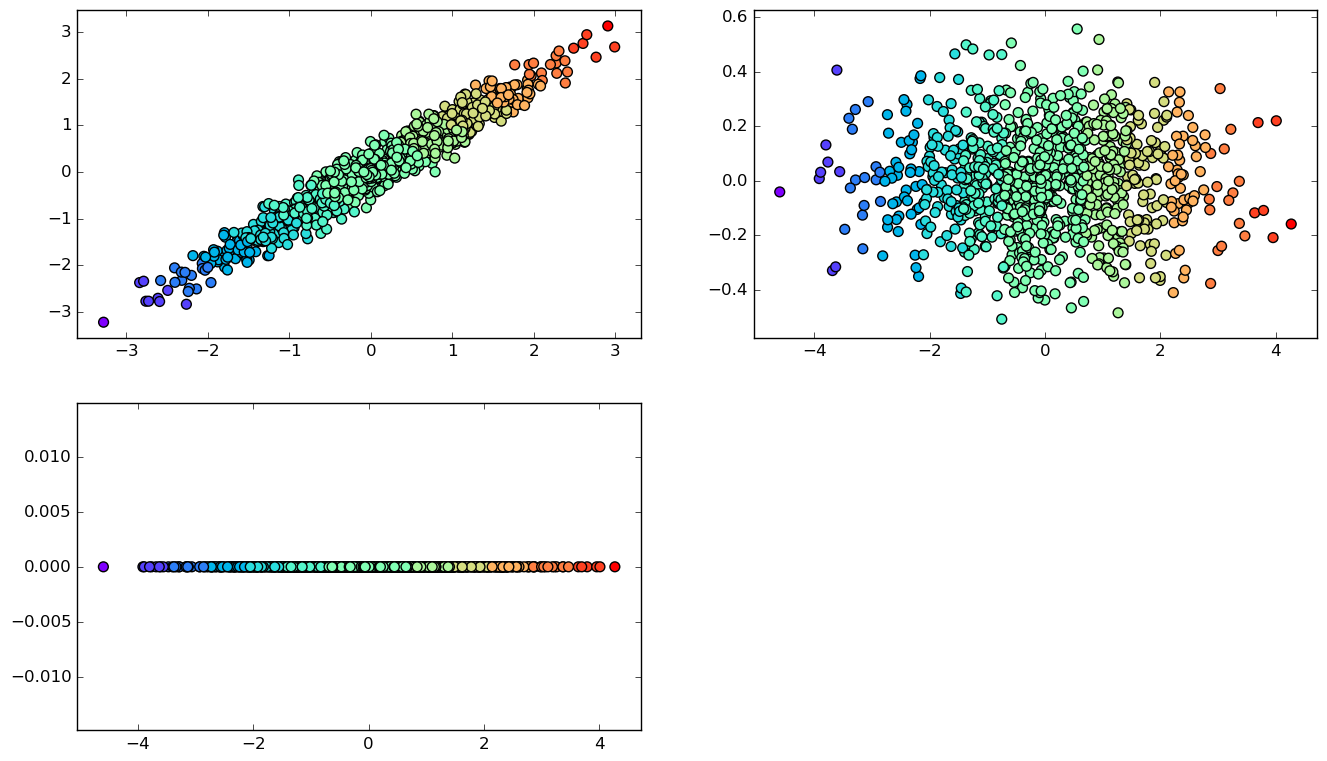
\includegraphics[width=.9\linewidth]{experiments/pca_r}
	\caption{The PCA algorithm reducing $K$ to 2 and 1 dimension, respectively.}
	\label{fig:datasetrpca}
\end{figure}

\begin{table}[H]
	\centering
	\begin{tabular}{|c|c|c|c|}
		\hline
		& \textbf{Original $\mathbb{R^2}$} & \textbf{$\mathbb{R}^2$} & \textbf{$\mathbb{R}$} \\\hline
		\textbf{Pred. accuracy} & .98 & .98 & .99 \\\hline
		\textbf{GridSearch time} & 1.15 s & .84 s & 1.26 s \\\hline
		\textbf{Reduction time} & - & 0.995 ms & 1.118 ms \\\hline
		\textbf{Stress} & - & 0 & .0399 \\\hline
		\textbf{Data size} & 15.62 KB & 15.62 KB & 7.81 KB \\\hline
	\end{tabular}
	\caption{Description of predictions and reduction performance for $K$.}
\end{table}

From the table above, one can also observe how Kruskal's stress might not be an appropriate quality measurement, given a specific domain. Indeed, for data set $K$, stress increase resulted from the removal of one of the components did not imply on prediction accuracy decrease.

\subsection{The Iris Flower Data Set}

The Iris flower from section \ref{irisdataset}, containing 150 samples and 5 features.

\begin{figure}[H]
	\centering
	\captionsetup{justification=centering}

	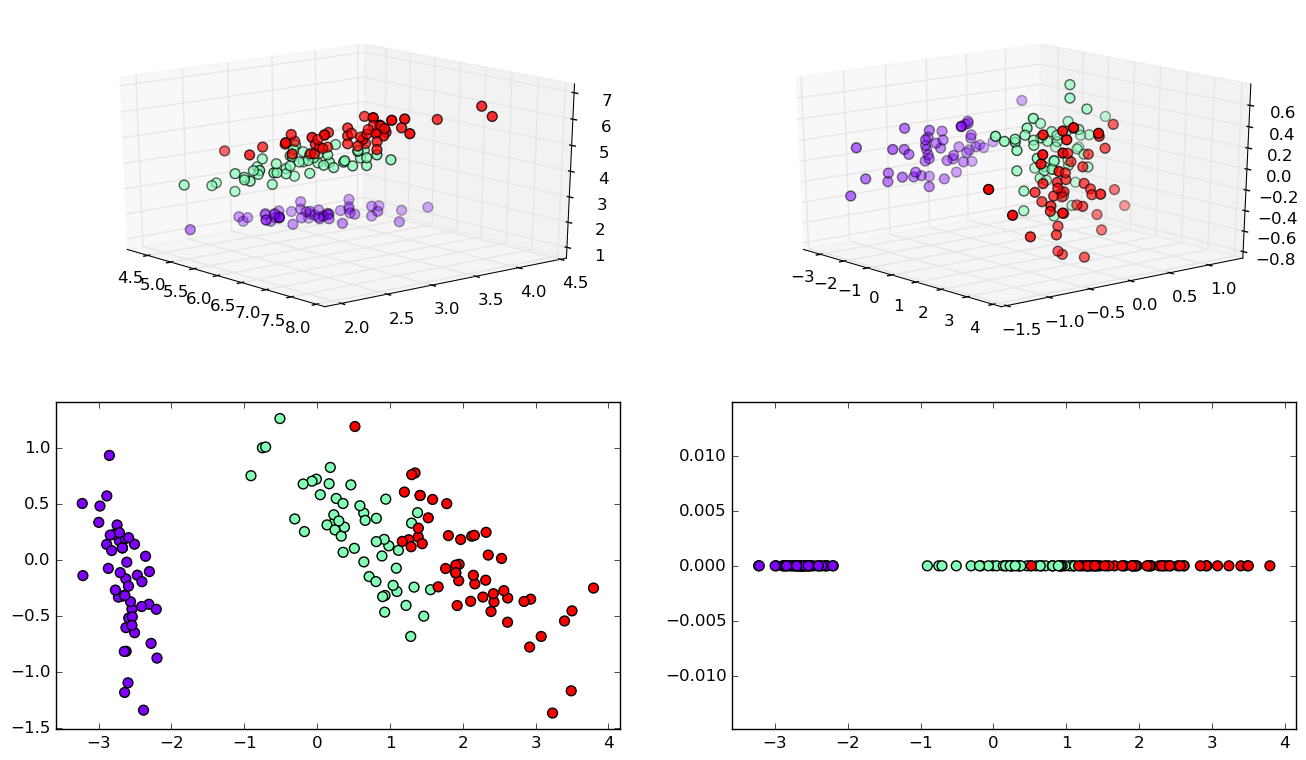
\includegraphics[width=\linewidth]{experiments/pca_iris}
	\caption{The Iris Flower data set and its reductions to 3, 2, and 1 dimensions, respectively.}
	\label{fig:dsirispca}
\end{figure}

Although the data set became nonlinearly separable, classes are still somewhat organized in different clusters.

\begin{table}[H]
	\centering

	\begin{tabular}{|c|c|c|c|}
		\hline
		& \textbf{Original data} & \textbf{Reduced data ($\mathbb{R}^2$)} & \textbf{Reduced data ($\mathbb{R}$)} \\\hline
		\textbf{Pred. accuracy} & .99 & .97 & .94 \\\hline
		\textbf{GridSearch time} & 1.71 s & 1.64 s & 1.78 s \\\hline
		\textbf{Reduction time} & - & 0.995 ms & 1.118 ms \\\hline
		\textbf{Stress} & - & .0418 & .1095 \\\hline
		\textbf{Data size} & 4.68 KB & 2.34 KB & 1.17 KB \\\hline
	\end{tabular}

	\caption{Description of predictions and reduction performance for Iris flower.}
\end{table}

\subsection{The Digits Data Set}

Digits data set is composed by 1797 samples, 64 features and 10 classes. Each sample is a 8x8 image of a hand-written digit from 0 to 9.

\begin{figure}[H]
	\centering
	\captionsetup{justification=centering}
	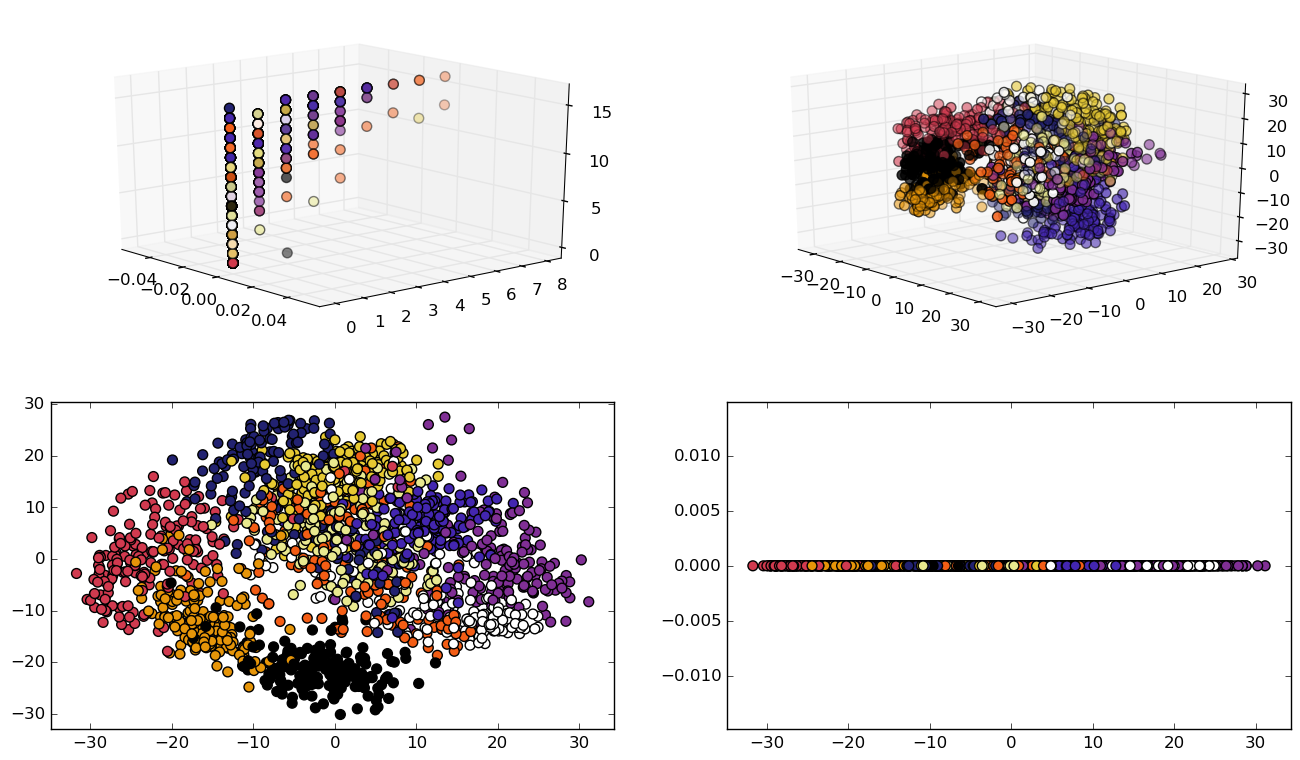
\includegraphics[width=\linewidth]{experiments/pca_digits}
	\caption{Digits data set reduced to 10, 3, 2 and 1 dimension, respectively.}
	\label{fig:dsdigitspca}
\end{figure}

\begin{table}[H]
	\centering
	\begin{tabular}{|c|c|c|c|c|c|}
		\hline
		& \textbf{$\mathbb{R}^{64}$} & \textbf{$\mathbb{R}^{10}$} & \textbf{$\mathbb{R}^3$} & \textbf{$\mathbb{R}^2$} & \textbf{$\mathbb{R}$} \\\hline
		\textbf{Pred. accuracy}   & .98 & .95 & .74 & .64 & .39 \\\hline
		\textbf{GridSearch time} & 8.51 s & 21.33 s & 151.04 s & 132.18 s & 113.78 s \\\hline
		\textbf{Reduction time} & - & 0.02 s & 0.01 s & 0.01 s & 0.01 s \\\hline
		\textbf{Stress} & - & .1594 & .4218 & .5405 & .7092 \\\hline
		\textbf{Data size} & 898.5 KB & 140.39 KB & 42.11 KB & 28.07 KB & 14.03 KB \\\hline
	\end{tabular}

	\caption{Description of predictions and reduction performance for Digits.}
\end{table}

Notice that it was possible to eliminate 54 dimensions, consistently reducing the data set size, and only suffering 3\% of prediction accuracy loss. The score drastically decreased, however, when more dimensions were removed. Furthermore, accuracy decrease was followed by stress increase.
